\section{1D 2G Homogeneous}
This problem is a simple version of a $k$-eigenvalue criticality problem using 1D, dual-energy diffusion for neutron transport.  While this problem is 1D, we use a 2D mesh to solve it by imposing reflecting boundary conditions on the top and bottom.  The governing PDE for this equation is
\begin{equation}
-\drv{}{x}D_g\drv{\phi_g}{x}+(\Sigma_{g,a}+\Sigma_{g,s})\phi_g = \sum_{g'}\sigma_{s}^{g'\to g}\phi_{g'} + \frac{\chi_{g}}{k}\sum_{g'}\nu_{g'}\sigma_{f,g'}\phi_{g'},\hspace{15pt} g\in[1,2],
\end{equation}
\begin{equation}
\Sigma_{g,a}=\Sigma_{g,\gamma}+\Sigma_{g,f},
\end{equation}
where $g$ denotes the energy group, $D$ is the group diffusion cross section; $\phi$ is the group flux, $x$ is the location within the problem; $\Sigma_a,\Sigma_s,\Sigma_f,\Sigma_\gamma$ are the macroscopic absorption, scattering, fission, and capture cross sections respectively; $k$ is the criticality factor eigenvalue and quantity of interest; and $\chi$ is the fraction of neutrons born into an energy group.  In this case, we consider only downscattering, and fission neutrons are only born into the high energy group ($\Sigma_s^{2\to1}=\chi_2=0$).

This problem does not have a convenient general analytic solution.  We can express the solver as
\begin{equation}
U(p;\theta) = k(p;\Sigma_{2,\gamma}),
\end{equation}
where
\begin{equation}
p=(D_g,\Sigma_{1,\gamma},\Sigma_{g,s},\nu_g,\Sigma_{g,f},\chi_g),\hspace{20pt}g\in[1,2].
\end{equation}
While $\phi_g(x)$ might also be considered a parameter, it is an output value solved simultaneously with $k$.

For this test code we consider $\theta=\Sigma_{2,\gamma}$ in three possible normal distributions.  Evaluated at the distribution mean of $\theta$, we consider one each case where $k=(0.9,1.0,1.1)$, given by the distributions $\theta\in\mathcal{N}(0.055969,0.1), \theta\in\mathcal{N}(0.04438,0.1), \theta\in\mathcal{N}(0.035181,0.1)$ respectively.

It is important to note that the Monte Carlo sampling was restricted to values within 3 standard deviations of the mean; as such, the means and variances obtained directly through Monte Carlo sampling are not representative of the full uncertainty space.  This truncation of the distribution is enforced because without such a restriction, it is possible to sample unphysical values for $\Sigma_{2,a}$, including negative values.

A summary of all three cases is shown in Fig. \ref{1d_all}.  Tabular data for mean and variance convergence is in Tables \ref{tab:1dcrit} to \ref{tab:1dsub}, where the clock time shown makes use of embarrassingly-parallel Monte Carlo sampling with 4 cores.  The times for the PCESC runs include the construction of the ROM prior to sampling.  The pdfs for each case are in Figs. \ref{fig:1d 3pdfs}.  

\begin{figure}[h!]
\centering
   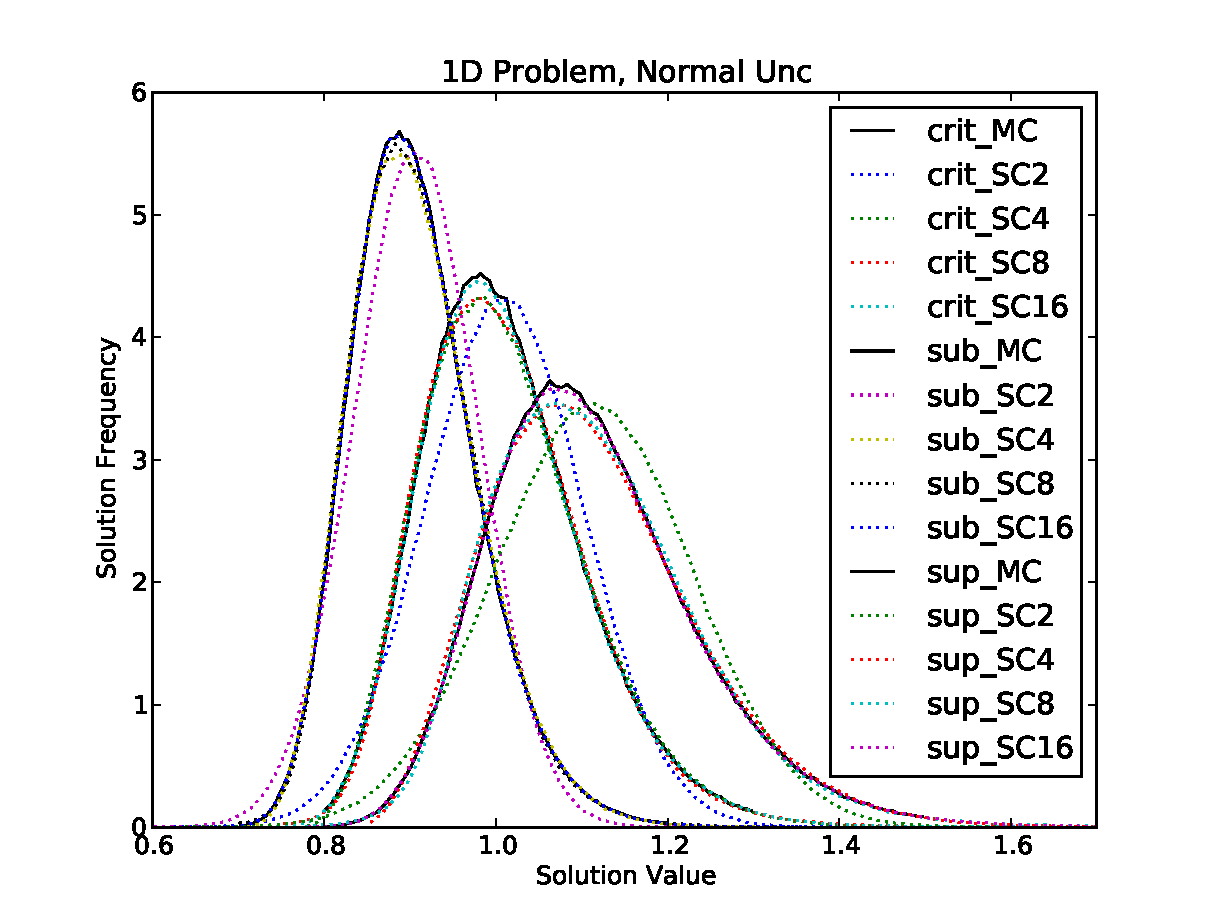
\includegraphics[width=.75\textwidth]{../graphics/1dall_normal_pdfs}
   \caption{Summary, 1D Criticality}
   \label{1d_all}
\end{figure}

\begin{table}
\begin{center}
\begin{tabular}{c c|l l l}
type & runs/order & mean & variance & time (s) \\ \hline
MC & $1\times10^6$ & 1.01144778738 & 0.0105716289269 & 15082  \\
SC & 2 & 1.01107577584 & 0.00974910361412 & 133 \\
SC & 4 & 1.0113755955 & 0.0105739848126 & 231\\
SC & 8 & 1.01137628238 & 0.0105785232446 & 450\\
SC & 16 & 1.01137628243 & 0.0105785241745 & 862
\end{tabular}
\end{center}
\caption{Convergence of Mean, Variance for Critical Case}
\label{tab:1dcrit}
\end{table}

\begin{table}
\begin{center}
\begin{tabular}{c c|l l}
type & runs/order & mean & variance \\ \hline
MC & $1\times10^6$ & 1.11593980088 & 0.0168503796482 \\
SC & 2 & 1.11537873568 & 0.0151539223359 \\
SC & 4 & 1.11590698755 & 0.016795821961\\
SC & 8 & 1.11590896034 & 0.0168106966474 \\
SC & 16 & 1.11590896088 & 0.0168107061554
\end{tabular}
\end{center}
\caption{Convergence of Mean, Variance for Supercritical Case}
\label{tab:1dsup}
\end{table}

\begin{table}
\begin{center}
\begin{tabular}{c c|l l}
type & runs/order & mean & variance \\ \hline
MC & $1\times10^6$ & 0.907699673282 & 0.00632790358771 \\
SC & 2 & 0.907653521565 & 0.00595095987773 \\
SC & 4 & 0.907813174929 & 0.00633526057266\\
SC & 8 & 0.907813389468 & 0.00633649118503 \\
SC & 16 & 0.907813389471 & 0.00633649126226
\end{tabular}
\end{center}
\caption{Convergence of Mean, Variance for Subcritical Case}
\label{tab:1dsub}
\end{table}

\subsection{Chaos Moment Quadrature Convergence}\label{sec:quadconv}
One concern with using stochastic collocation to build the polynomial chaos moments is the appropriate order of quadrature to use.  With Gaussian quadrature, a sum with $n$ terms can exactly integrate a polynomial of order $2n-1$.  The chaos moment expression we integrate is
\begin{align}
c_i &= \int_\Omega U(\theta)P(\theta)B_i(\theta)d\theta,\\
  &\approx \sum_{\ell=0}^L w_\ell U(\theta_\ell)B_i(\theta_\ell),
\end{align}
where $P$ is the probability distribution of $\theta$ and $B_i$ is the $i-th$ order basis polynomial.  In the simplest case when $U(\theta)$ is a scalar quantity, the order of the expression under the integral is determined solely by the basis polynomial.  Thus a quadrature order of $(i+1)/2$ is the minimum quadrature order necessary to integrate the chaos moments.  In the case $U(\theta$) is highly nonlinear and ill-approximated by even high-order polynomials, the necessary quadrature order required to accurately determine moments is much higher.

As an example of chaos moment convergence as a function of quadrature order, we show the PCESC moments of the critical case for 7th-order quadrature in Table \ref{tab:quadconverge}, as determined by increasing orders of quadrature from the minimum to 12-th order, which assumes $U(\theta)$ is well-approximated by a 7th-order polynomial.  As can be seen, the lower moments require smaller quadrature orders, and at least order 8 quadrature is necessary to see reasonable convergence for higher moments.  In addition, the moments calculated using quadrature order equal to expansion order are given for expansion orders 2 to 32 in Fig. \ref{tab:1dcrit coeffs}.
\begin{landscape}
\begin{table}[H]
\begin{center}
\begin{tabular}{c | *{8}{l}}
Quadrature Order & $c_0$ & $c_1$ & $c_2$ & $c_3$ & $c_4$ & $c_5$ & $c_6$ & $c_7$ \\ \hline
5 & 1.34648094 & -0.13502447 & 0.02226791 & -0.0045477 & 0.00000000 & 0.00101863 & -0.00092988 & 0.00313821\\
6 & 1.34648100 & -0.13502501 & 0.02227125 & -0.00456451 & 0.0010908 & -0.00027317 &  0.00000000 & 0.00025291\\ 
8 & 1.34648101 & -0.13502506 & 0.02227158 & -0.00456614 & 0.0010978 & -0.00029964 & 9.01120742e-05 & -2.67010906e-05\\ 
10& 1.34648101 & -0.13502506 & 0.02227158 & -0.00456616 & 0.0010979 & -0.00030000 & 9.13419949e-05 & -3.05173759e-05\\ 
12& 1.34648101 & -0.13502506 & 0.02227158 & -0.00456616 & 0.0010979 & -0.00030001 & 9.13732306e-05 & -3.06142832e-05
\end{tabular}
\end{center}
\caption{Chaos Moment Convergence with Increasing Quadrature Order}
\label{tab:quadconverge}
\end{table}
\vspace{50pt}
\begin{figure}[H]
\centering
\begin{subfigure}[b]{0.43\textwidth}
   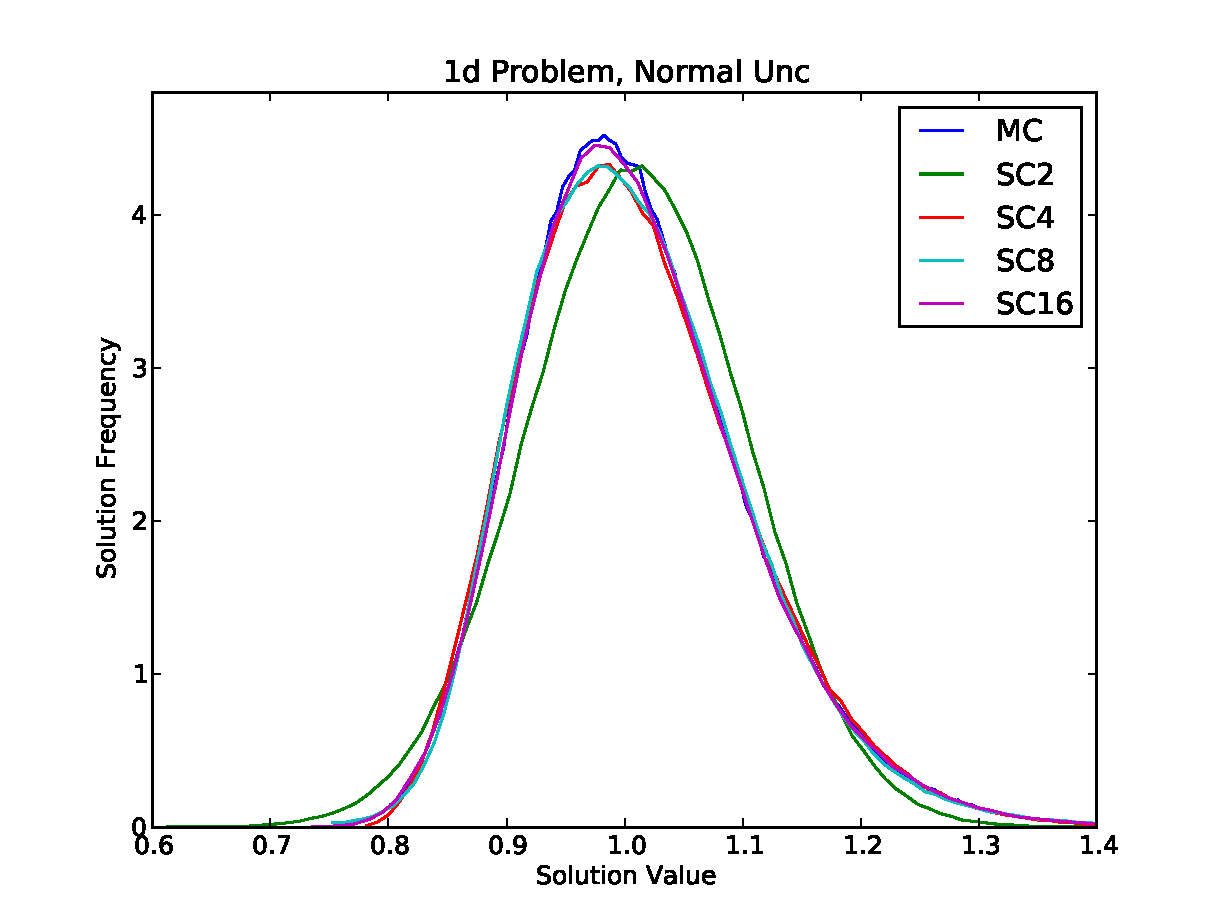
\includegraphics[width=\textwidth]{../graphics/1d_normal_pdfs}
   \caption{Critical}
   \label{fig:1dcrit}
\end{subfigure}
\begin{subfigure}[b]{0.43\textwidth}
   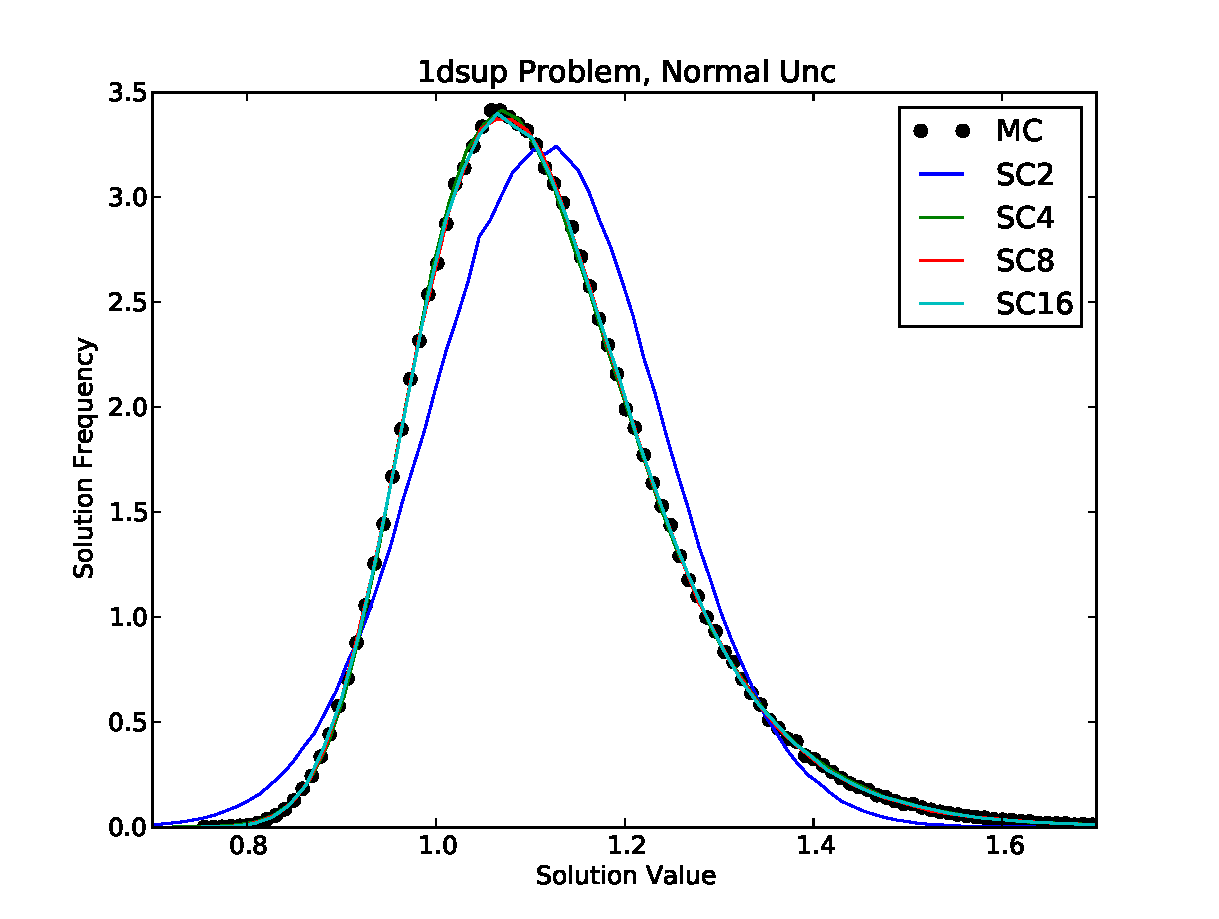
\includegraphics[width=\textwidth]{../graphics/1dsup_normal_pdfs}
   \caption{Supercritical}
      \label{fig:1dsup}
\end{subfigure}
\begin{subfigure}[b]{0.43\textwidth}
   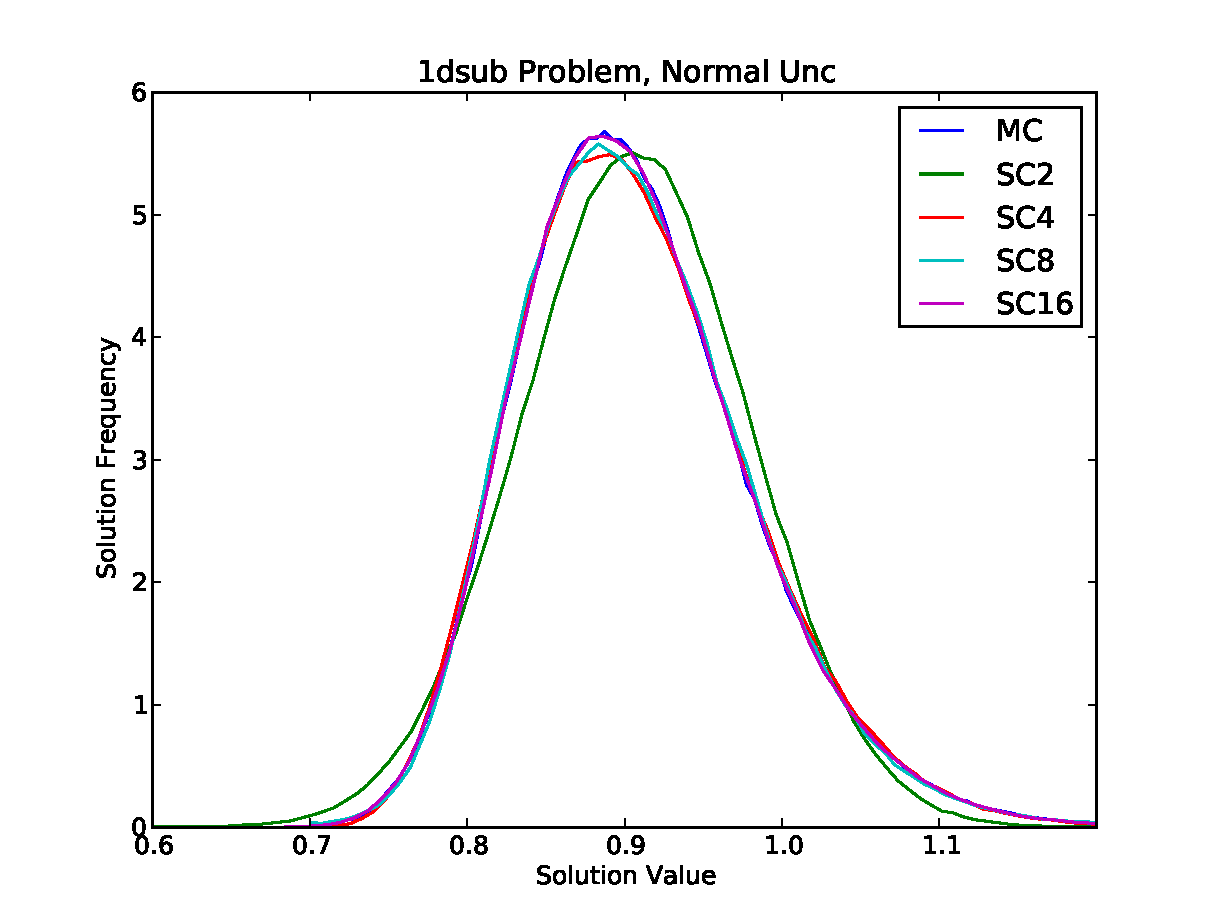
\includegraphics[width=\textwidth]{../graphics/1dsub_normal_pdfs}
   \caption{Subcritical}
      \label{fig:1dsub}
\end{subfigure}
\caption{1D Solution PDF Convergences}
\label{fig:1d 3pdfs}
\end{figure}
\end{landscape}

\begin{table}[H]
\begin{center}
\begin{tabular}{c | l l l l l}
Moment & SC1 & SC3 & SC7 & SC15 & SC31\\ \hline
0 & 1.34608094 & 1.3464801 & 1.34648101 & 1.34648101 &  1.34648101\\
1 & -0.13145279 & -0.1350169 & -0.13502506 & -0.13502506 &  -0.13502506\\ 
2 & 0 & 0.02222067 & 0.02227158 & 0.02227158 &  0.02227158\\ 
3 & 0 & -0.00431037 & -0.00456614 & -0.00456616 & -0.00456616 \\ 
4 & 0 & 0 & 0.0010978 & 0.0010979 & 0.0010979 \\ 
5 & 0 & 0 & -0.00029964 & -0.00030001 & -0.00030001 \\ 
6 & 0 & 0 & 9.01120742e-05 & 9.13747084e-05 & 9.13746830e-05 \\ 
7 & 0 & 0 & -2.67010906e-05 & -3.06188612e-05 & -3.06187650e-05 \\ 
8 & 0 & 0 & 0 & 1.11868181e-05 & 1.11865704e-05 \\ 
9 & 0 & 0 & 0 & -4.42800671e-06 & -4.42735312e-06 \\ 
10 & 0 & 0 & 0 & 1.89021407e-06 & 1.88853134e-06 \\ 
11 & 0 & 0 & 0 & -8.66874281e-07 & -8.62852707e-07 \\ 
12 & 0 & 0 & 0 & 4.24658199e-07 & 4.15693998e-07 \\ 
13 & 0 & 0 & 0 & -2.18790217e-07 & -1.99976426e-07 \\ 
14 & 0 & 0 & 0 & 1.12938059e-07 & 7.56801496e-08 \\ 
15 & 0 & 0 & 0 & -4.90000878e-08 & 2.05894301e-08 \\ 
16 & 0 & 0 & 0 & 0 & -1.22580841e-07 \\ 
17 & 0 & 0 & 0 & 0 & 2.51097599e-07 \\ 
18 & 0 & 0 & 0 & 0 & -4.18278488e-07 \\ 
19 & 0 & 0 & 0 & 0 & 6.25910592e-07 \\ 
20 & 0 & 0 & 0 & 0 & -8.61060458e-07 \\ 
21 & 0 & 0 & 0 & 0 & 1.09209939e-06 \\ 
22 & 0 & 0 & 0 & 0 & -1.26866179e-06 \\ 
23 & 0 & 0 & 0 & 0 & 1.32892404e-06 \\ 
24 & 0 & 0 & 0 & 0 & -1.21597330e-06 \\ 
25 & 0 & 0 & 0 & 0 & 9.01437926e-07 \\ 
26 & 0 & 0 & 0 & 0 & -4.09433059e-07 \\ 
27 & 0 & 0 & 0 & 0 & -1.70599526e-07 \\ 
28 & 0 & 0 & 0 & 0 & 6.94034499e-07 \\ 
29 & 0 & 0 & 0 & 0 & -9.99892578e-07 \\ 
30 & 0 & 0 & 0 & 0 & 9.71463606e-07 \\ 
31 & 0 & 0 & 0 & 0 & -5.97051529e-07 \\ 
\end{tabular}
\end{center}
\caption{Chaos Moments for 1D Critical Case}
\label{tab:1dcrit coeffs}
\end{table}
%
%\begin{figure}[h!]
%\centering
%   \includegraphics[width=\textwidth]{../graphics/}
%   \label{}
%   \caption{}
%\end{figure}
%\begin{table}
%\begin{center}
%\begin{tabular}{c c|l l| r}
%type & runs/order & mean & variance & run time (sec) \\ \hline
%MC & 1\times10^6 &  &  & \\
%SC & 2 & & & \\
%SC & 4 & & & \\
%SC & 8 & & & \\
%SC & 16 & & &
%\end{tabular}
%\end{center}
%\caption{}
%\label{}
%\end{table}
%
%\begin{figure}[h!]
%\centering
%   \includegraphics[width=\textwidth]{../graphics/}
%   \label{}
%   \caption{}
%\end{figure}
